% !TEX root = Projektstudie.tex
% Einleitung

\section{Einleitung}

Der Mecanum-Roboter ist ein omnidirektionales Fahrzeug. Er kann jederzeit aus jeder Position in eine beliebige Richtung fahren. Grund dafür sind die verwendeten Allseitenräder - Mecanum-Räder - auf deren Umlauffläche 15 weitere tonnenförmige Hilfsräder angebracht sind. Zur Steuerung des Roboters ist es notwendig ein mathematisches Modell zur Beschreibung der einzelnen Bewegungen der Räder aufzustellen. Ziel ist es eine Kreisfahrt zu programmieren. 

Bisher werden die Schrittmotoren der Räder mit Hilfe von Nanotec-Treiberkarten und dem CANopen Protokoll angesteuert. Das CANopen Protokoll nutzt als Übertragungsmedium den CAN-Bus.  Die Kommunikation läuft über eine SPS. Diese soll aus Kostengründen durch einen Arduino mit einem CAN-Shield ersetzt werden. Der Austausch soll zudem die Programmierung der Bewegung des Mecanum-Roboters erleichtern.

Zusammengefasst ist es das Ziel der Projektstudie den Austausch zu realisieren, die Bewegung des Roboters über den Arduino zu programmieren und den Roboter über einen Joystick zu steuern. Die omnidirektionale Kinematik soll zudem durch einen Simulator verdeutlicht werden. Die Programmierung dessen soll ebenfalls umgesetzt werden.


\begin{figure}[H]
\centering
 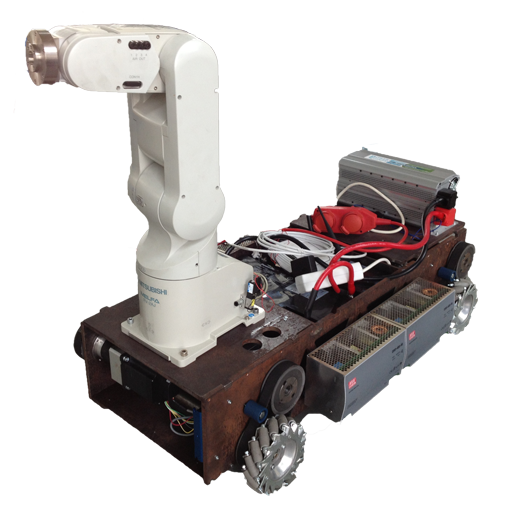
\includegraphics[width=.6\textwidth]{Abbildungen/Roboter} 
\caption[Mecanum-Roboter]{Mecanum-Roboter.}
\label{fig:Roboter}
\end{figure}


Der Mecanum-Roboter ist 1000 mm lang. Er ist mit vier Mecanum-Rädern, die im Rechteck angeordnet sind, ausgestattet. Der Radstand beträgt 775 mm und die Spurbreite beträgt 490 mm. Die Räder haben einen Durchmesser von 115 mm und besitzen jeweils 15 Hilfsrollen. Eine detaillierte Beschreibung folgt im Kapitel \ref{sec:Mecanum-Räder}.

Die Anordnung der Mecanum-Räder und deren Technologie ermöglichen dem Mecanum-Roboter eine omnidirektionale Bewegung. Er kann sich ohne mechanische Lenkung aus jeder Position in jede Richtung fortbewegen.

\subsection{Mecanum-Räder}
\label{sec:Mecanum-Räder}
Das Mecanum Rad wurde 1973 von der schwedischen Firma Mecanum AB entwickelt und bedient unter-schiedliche Anwendungen. Heutige Anwendungsbeispiele sind unter anderem Förderfahrzeuge, fahrerlose Transportfahrzeuge oder Mobilitätshilfe. Auch in der Robotik finden die Allseitenräder immer häufiger Verwendung.
\begin{figure}[H]
\centering
 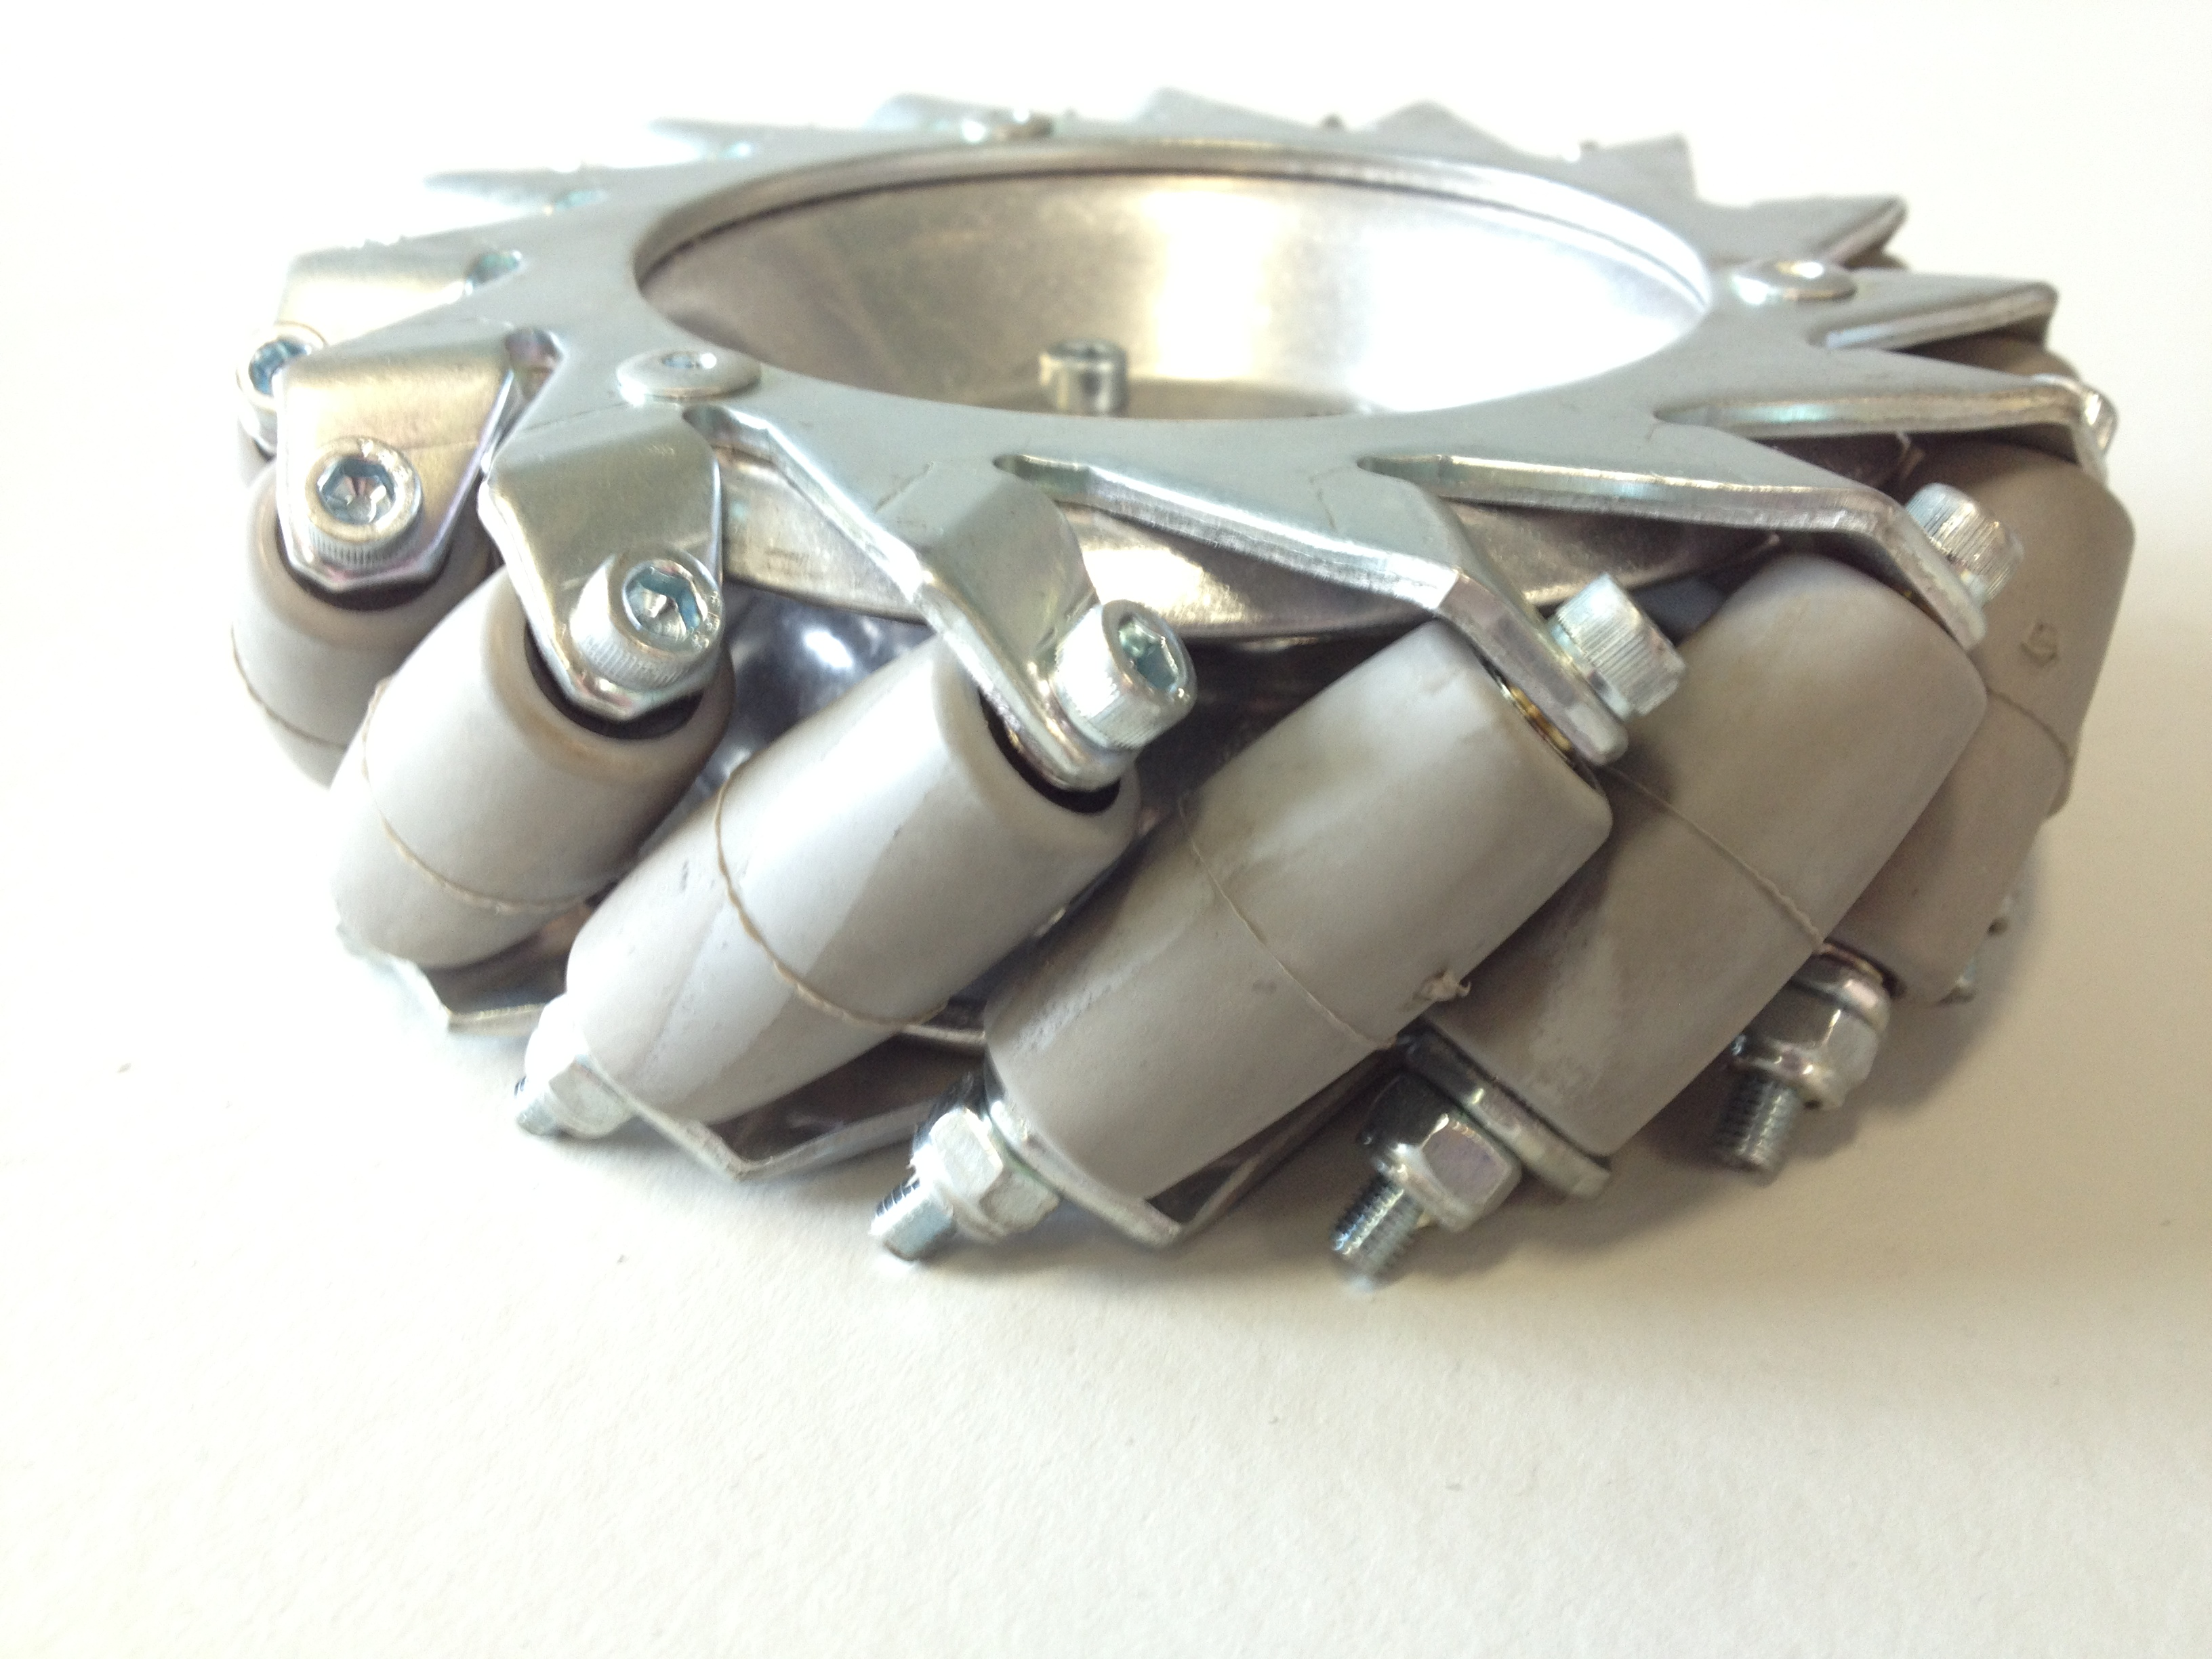
\includegraphics[width=.6\textwidth]{Abbildungen/Mecanumrad} 
\caption[Mecanum-Rad]{Mecanum-Rad.}
\label{fig:Mecanum-Rad}
\end{figure}
Abbilung \ref{fig:Mecanum-Rad} zeigt ein Mecanum-Rad des Mecanum-Roboters. Auf dem Umfang des Rades sind 15 tonnen-förmige beschichtete Rollen im Winkel von 45 Grad zu Radachse angebracht. Diese Rollen haben keinen eigenen Antrieb und sind frei drehbar gelagert. Ausschließlich die Rollen haben Kontakt zum Boden.
Jedes Mecanum-Rad wird von einem Schrittmotor angetrieben. Somit sind Drehsinn und Drehzahl für jedes Rad einzeln ansteuerbar. Dieses ist entscheidend für die omnidirektionale Bewegung.
Durch eine individuelle Drehrichtungsauswahl entstehen durch die Hilfsrollen am Untergrund Kraftvektoren in unterschiedliche Richtungen. Die Summe der Vektoren aller Räder bildet die Gesamtbewegungs-richtung oder auch ein Gesamtdrehmoment.